\documentclass[12pt]{article}
\usepackage{url}
\usepackage[authoryear,round]{natbib}
\usepackage{graphicx} 

%%FIXME: I would use some markup for the package name(s)

\title{Outline flowCore paper}


\author{Florian Hahne*\\
  Nolwenn LeMeur*\\
  Byron Ellis\\
  Ryan Brinkman\\
  Perry Haaland\\
  Errol Strain\\
  Deepayan Sarkar\\
  Josef Spidlen\\
  Robert Gentleman
 }

\begin{document}

\maketitle

\section*{Introduction}
\subsection*{Computational tools for the analysis of FC-HCS data}
During the last several years, automation technologies have been
developed that enable the use of flow cytometry high content screening
(FC-HCS) to generate large, complex datasets in both basic and
clinical research applications \citep{brinkman2007hcf}. A serious
bottleneck in the interpretation of existing studies and the
application of FC-HCS to even larger, more complex problems is that
data management and data analysis methods have not advanced
sufficiently far from the methods developed for traditional
small-scale, tube-based studies.
%%FIXME: RG
%applications of flow cytometry (FCM) to small-scale, tube-based
%studies.

Some of the consequences of this lag in development are difficulties
in maintaining the integrity and documentation of extremely large
datasets, assessing measurement quality, developing validated assays,
controlling the accuracy of gating techniques, automating complex gating
strategies, and aggregating statistical results across large study
sets for further analysis.  Among the most serious consequences of the
current situation is, however, that it is very difficult for new
analysis approaches to find there way into standard practice. We
believe that this barrier to the development and dissemination of new
analysis methods is one of the fundamental restraints on the future
expansion of FC-HCS in both clinical and research applications.

In this paper, we describe a set of flexible and well structured
computational tools to efficiently analyze FC-HCS. This set of tools
is based on the open source statistical software R \citep{Rmain}, in
conjunction with the Bioconductor Project \citep{BIOC}. Our intent is
to provide a shared research platform that enables bioinformaticians,
computer scientists, and statisticians to work collaboratively with
biologists and clinicians to develop novel methods  
%%this reference is a bit odd here - you better explain what they say
%%and why you quote them 
\citep{lizard2007fca} for FCM data analysis. A critical component of
this approach is the development and implementation of standards that
will facilitate the adoption of these methods by both the larger
research community and commercial software vendors.  Consequently, we
are optimistic that this software platform will play a critical role
in addressing the bottlenecks described above that limit further
advances in the application of FC-HCS.

The computational tools we have developed are distributed in the R
software language as the Bioconductor package flowCore. flowCore is a
freely available, highly functional and extensible FCM data analysis
platform that enables researchers to efficiently handle FC-HCS data
and encourages open development of tools for their coherent
analysis. Among the issues addressed by flowCore are computationally
efficient data structures and a range of specialized methods for
compensation, transformation, and gating.  flowCore runs on Windows,
Mac OS X and Linux/Unix operating systems. Conceptually, the
underlying data structures that build the core of our software can be
implemented in any programming language, and we chose the R language
for its advantages in statistical programming and visualization. In
this paper, we describe the functionality and methods underlying
flowCore, and provide examples of their use.

\subsection*{R and Bioconductor}
R is a robust statistical programing environment which offers a wide
range of statistical and visualization methods developed for various
fields of application. In particular, the Bioconductor project
provides R software modules for biological and clinical data analysis.
It is widely used to process such data, spanning a diversity of
research fields including genomics, proteomics and cell biology
\citep{gentleman2006bos}. The R language and Bioconductor are
particularly geared towards the analysis of large complex datasets
that typically arise from high throughput experiments such as
microarray gene expression analysis or FC-HCS. Using flow cytometry as
a high-throughput technology requires suitable software infrastructure
to facilitate the rapid handling of the data. In our implementation of
flowCore we rely on two important lessons learned from the field of
gene expression data analysis: the first being the importance of data
structures that reflect the underlying data and facilitate the
manipulations that are of most interest, while the second is the
importance of a modular architecture that allows for many developers
to extend and use the underlying infrastructure and to combine tools
in complex work flows.

\subsection*{Existing data standards and conventions}
%%FIXME: I think that this section is mixing two ideas - the need for
%%data representation - eg the class hierarchy, and the analysis
%%tools. RG suggests starting by saying what they do -then point out
%%that for complex experiments there is data on the samples (time
%%points, drugs etc - we have examples to cite) and the need to
%%combine these.  The notion of classes from an OOP language provide
%%one coherent way to describe these richer data structures and
%%functions/methods can work on them.  We will describe the classes
%%and their implementation in R, but they could just as easily be
%%written in any other language (eg Java, C++), and if
%%programs/analysis tools written in those languages use similar
%%structures then communication is simplified, and users could more
%%easily move data between analysis tools.  I doubt that reflection is
%%needed here - but if so, it would allow a naive function to get
%%information about the data structure (it is hard for it to use that
%%information though)

Currently, data from FCM experiments are stored in single files
according to the Flow Cytometry Standard (FCS) \citep{seamer1997pnd}.
However, recent developments in high-throughput FCM are shifting the
focus of interest away from single-tube based measurements towards
large and complex experimental designs with dozens of covariates and
influencing factors. Self-contained reflective data
%%FIXME: might need to explain reflective - or at least how you are
%%going to use this - we may need a graphic that shows the flow data,
%%data about the dyes antibodies but also about the samples etc - and
%%the need to keep this coordinated through an analysis
structures are a prerequisite to allow for coordinated analysis of
such experiments.  Many of the currently available software solutions
offer only limited support for such structures, or make use of
containers like XML or binary storage formats that are designed
specifically for particular user interfaces and hence are not easily
amenable to programmatical access. In addition, the closed-source
nature of these products often makes it impractical to integrate them into
analysis pipelines.

Traditionally, the majority of FCM experiments have been analyzed by
manual data inspection in one or two dimensions, or by very basic
comparisons of summary statistics. We believe that these approaches,
in addition to being extremely expensive and labor intensive, do not
fully address the highly complex nature of FCM data; in particular,
they discard many of the fundamental aspects of the data, such as its
underlying distribution and its high-dimensional nature. Furthermore,
the subjective character of manual analyses are a major obstacle to
reproducibility. For FC-HCS data, unassisted manual inspection is
extremely time consuming, and robust statistical methods need to be
developed to point investigators to interesting aspects of the data,
or to potential problems. While the expert knowledge of immunologists
and researchers remains crucial for the understanding of FCM data, we
believe that collaboration with other research fields such as
statistics and computer science can greatly improve the relevance of
FCM in today's high-throughput paradigm.

These issues are currently being addressed by emerging new flow
cytometry data standards developed in collaboration with the ISAC Data
Standards Task Force.  For example, the Gating-ML Candidate
Recommendation (CR) \textit{Fixme Ryan or Joseph: How do we cite
  this?}  represents a proposal on how to form unambiguous XML-based
gate definitions, which can facilitate the interchange and validation
of data between different software packages. Gates may be ordered into
a hierarchical structure to describe a gating strategy. This enables
the encoding of a simple analytical work flow, in a way that allows us
to reconstruct the analysis programmatically.

The flowCore framework presented here can import raw data FCS files
along with their complete set of file-specific meta information
(Figure~\ref{fig1:FrameWork}).  Moreover, it is a software
implementation of the Gating-ML CR, which makes it possibile to
integrate flowCore in existing work flows and to communicate with
any other FCM tool that adheres to the proposed standard. Adherence
to standards also plays a critical role in the ability of new methods
based on flowCore to find there way back into the standard practices
for FCM data analysis.  Note that the data structures defined in
flowCore aim to model large sets of FCM data in a natural and coherent
way; they are not specific to the R language and can be implemented in
any other programming language. Ideally, different software programs
would communicate on the level of these data structures rather than a
high-level markup language.

%%FIXME: class hierarchy is probably not going to be well understood
%%by readers - you might need to work that into a more coherent
%%general discussion
flowCore is not a GUI-driven software, and all operations are done
using a command line interface.  It is possible to add a more
elaborate user interface on top of this infrastructure, however the
focus in this paper is on a programmatic approach to enable the
convenient development of novel analysis methods and automation of
complex analysis approaches.  By taking the burden of data management
from the programmer, and by providing well-defined programming
interfaces (APIs) and a structured class hierarchy, it is possible to
readily test new ideas and to easily extend the framework's
functionality.



\section*{Materials and Methods}
\subsection*{Basic data structures}
\subsubsection*{flowFrame}

FlowCore's primary task is the representation and basic manipulation
of FCM data. This is accomplished through a data model very close to
that adopted by other Bioconductor packages. All information from a
single FCS file, i.e., the collection of events and the accompanying
meta data, is stored in one single container. We call the structure
that hold this data a flowFrame. Raw data values as well as associated
metadata of a flowFrame can be accessed programmatically. Most
commonly, the metadata consist of descriptors of the stains used in
the experiment and the respective measurement channels, information
about compensation performed at the instrument side and any additional
keywords the user deems to be important to annotate the data. A number
of quality checks are performed during the creation of a flowFrame to
ensure data integrity.

%%again some markup for the class names would help the reader
%% stick with annotation or metadata not both
\subsubsection*{flowSet}
In high-throughput FCM, many of the analysis tasks need to be
performed consistently across multiple flow measurements, hence we
introduce the concept of a collection of flowFrames called a
flowSet. A flowSet is a container for multiple flowFrames along with
relevant information associated with each individual frame such as
descriptions of the cell sample, the treatment to which the sample was
subjected, or the location of that sample in a 96 or 384 well plate.
FlowSets manage the consistent application of operations on the
individual flowFrames and shift the burden of keeping score of the
annotation from the user to the infrastructure, thus reducing the risk
of errors (\textit{e.g.}, mixups of sample labels). The flowSet
structure can be readily extended to incorporate the potentially
complex annotation associated with even larger FC-HCS experiments such
as clinical trials where hundreds patients might provide samples at
different points in time over the course of the experiment.  Access to
flowCore data structures and methods has already enabled the
development of new Bioconductor packages, such as plateCore, that
facilitate the analysis of plate-based FC-HCS data and make handling
the annotation and processing the data easier.


%%Figure1 Diagram of the data structures and the basic operations
\begin{figure}
\centering
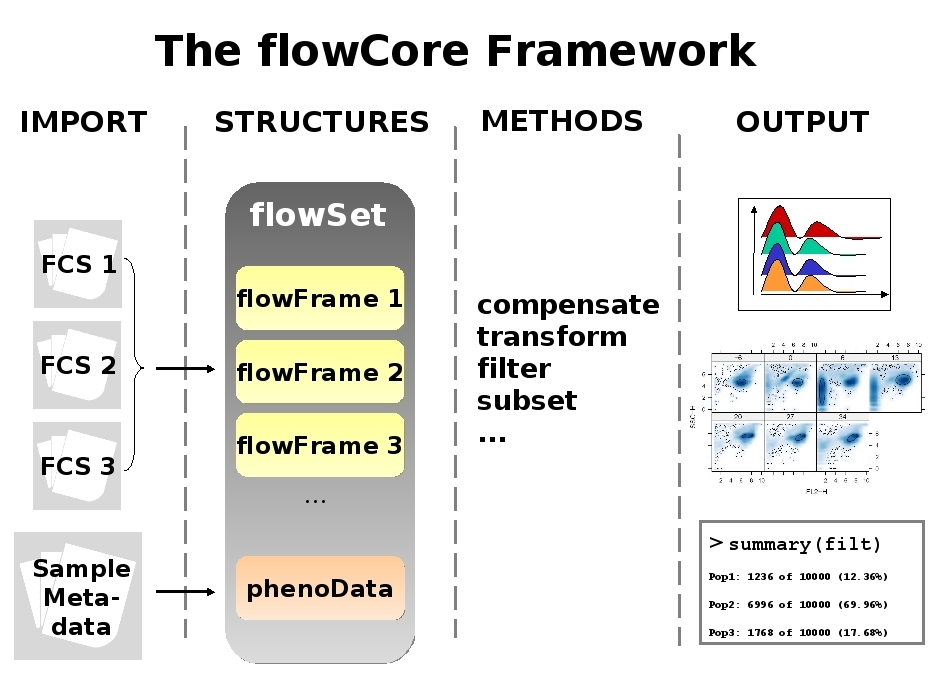
\includegraphics[width=0.9\textwidth]{Figure1-flowCoreFrameWork.jpg}
\caption{\label{fig1:FrameWork}{For each experiment, FCS files (as
    individual flowFrames), phenotypic and meta data are stored in a
    flowSet. Each flowFrame in a flowSet corresponds to one FCS
    file. All basic operations (e.g., compensation, transformation,
    gating) can be applied to either single flowFrames or a flowSet
    simultaneously.}}
\end{figure}

%%FIXME: if possible I would make the box that has Sample Meta-data in
%%it, be more of a table view (Age Sex Time with numbers and then it
%%might be more obvious what is happening


\subsection*{Standard flow operations}

The basic operations in FCM analyses are typically the same: the data
need to be compensated (if that was not already done on the instrument)
and transformed, and sup-populations of interest need to be selected
based on a set of (predominantly sequential) gates. All software
solutions for FCM analysis offer support for
these operations, typically in an interactive, GUI-driven interface. The
approach we have taken in flowCore is to abstractly describe these
operations and build a set of tools to perform them on both flowFrames
and flowSets. While transformation, and to a certain extent
compensation, are fairly routine operations with only limited
potential for improvement, being able to implement new methodologies
for gating of FCM data, and extending the capabilities of flowCore
through object oriented programming are features that clearly sets our
framework apart from other FCM analysis tools. By factoring out as
much of the bookkeeping as possible, programmers can focus on the
actual operations rather then having to deal with the tedious details
of data integration and access. Third-party methods can act on their
own as first-class citizens in the analysis framework, without
breaking the work flow or the basic infrastructure. This design allows
for the straightforward extension of flowCore's capabilities, and has
already fostered the development of a number of valuable add-ons
\citep{lo2008agf,sarkar2008ufv} \textit{(Fixme Errol: Will plateCore
  be in Bioconductor soon. It should be if we want to cite it.)}.

\subsubsection*{Transformation and compensation}

Data transformation is essential for both data visualization and
modelling \citep{lo2008agf}. The major transformations that are
routinely used in FCM analysis have been implemented in flowCore
(\textit{e.g.,} quadratic, log or arcsinh, see Table~\ref{table1} for a
complete list). Furthermore, the design of the R language makes it
easy to define arbitrary functions to apply to the data of individual
flowFrames or entire flowSets, respectively. Compensation is
available for both flowFrames and flowSets, and the software also
offers functionality to compute spillover or compensation matrices
from a set of appropriate compensation samples.

\begin{table}[ht]
\begin{center}
\begin{tabular}{|l|l|}
\hline
\multicolumn{2}{|c|}{Data Transformations} \\
\hline
linear & $ax + b$ \\
quadratic & $ax^2 + bx + c$ \\
natural logarithm & $ln(x)(r/d)$ \\
logarithm & $log(x)(r/d)$ \\
biexponential & need equation \\
logicle& need equation \\
truncate & $x_{x<=a} = a$ \\
scale & $(x-a)/(b-a)$ \\
split-scale & combination of linear and logarithm \\
arcsinh & $asinh(a + bx)+c$ \\
\hline
\end{tabular}
\caption{\label{table1}Data transformations implemented in flowCore.}
\end{center}
\end{table}

\subsubsection*{Gating}
%%FIXME: I would make more of the filters and possibly try to make it
%%clearer how much stuff thre is for composition of gates/filters etc
%%
%% somewhere notions of apply and summary methods should appear and if
%% we have anything figured out yet on how to do the subsetting etc
%% that too would go nicely in here (here I am thinking of our
%% discussion of the sort of workflow stuff)

In flowCore, gating operations are represented by classes that can be
extended in an object-oriented manner (Table~\ref{table2}). Basic gate
types such as rectangular gates, ellipses and polygon gates are
implemented as part of the framework. In addition, we introduce the
notion of data-driven gates, or filters, for which the necessary
parameters are computed based on the properties of the underlying
data, for instance by modelling data distribution or by density
estimation. The ability to programmatically access gates is a
prerequisite for automated or semi-automated gating. By utilizing a
unified interface for all different types of gates, the user is able
to subset data sets as well as to create summary statistics, for
example the proportions of events falling in a single gate or in a
combination of gates. Complex combinations and hierarchies of gates
can be captured in objects of class filterSet, allowing to apply
multi-step gating strategies. The definition of gates in flowCore
follows the Gating-ML CR, thus any flowCore gating strategy can be
reproduced by any other software that also adheres to the standard.

\begin{table}[ht]
\begin{center}
\begin{tabular}{|l|l|}
\hline
\multicolumn{2}{|c|}{Gates} \\
\hline
rectangleGate & n-dimensional rectangular regions \\
quadGate & quadrant regions in two dimensions \\
polygonGate & polygonal regions in two dimensions \\
polytopeGate & generalization of polygon in n dimensions \\
ellipsoidGate & n-dimensional ellipsoid region \\
\hline
\multicolumn{2}{|c|}{Filters} \\
\hline
sampleFilter & random sub-sampling\\
expressionFilter & results of a boolean expression \\
kmeansFilter & K-means clustering \\
norm2Filter & bivariate normal distribution \\
curv1Filter & local density regions in 1D \\
curv2Filter & density regions in 2D \\
timeFilter & abnormal data acquisition over time \\
\hline
filterSet & gating strategies \\
\hline
\end{tabular}
\caption{\label{table2}Filter and gate classes implemented in flowCore.}
\end{center}
\end{table}

\subsection*{Related flow packages}

In addition to the flowCore package that offers basic infrastructure,
we have implemented a range of additional Bioconductor packages that
are dedicated to more specific tasks of FCM data analysis. The flowViz
package \citep{sarkar2008ufv} provides sophisticated data
visualization tools, that make use of multivariate trellis plotting
\citep{FIXME:citeDeepayansBook}.  These functions can be used to
quickly generate customized plots for extended cytometry data sets for
both direct data inspection and quality control.  The objects
annotation information can be used to arrange the layout and
composition of the plots.  Furthermore, the design and the API of the
visualization software is very generic, and users can readily extend
its capabilities by providing self-defined plotting functions.  The
flowQ package offers more advanced quality assurance (QA) methodology
and a framework to create interactive web-based reports of QA results.
Most of flowUtil's content deals with data import and export using the
flow-cytometry specific standard markup languages (FIXME:it implements
the standards doesn't it?).  Finally, flowStats provides more
elaborate statistical methods that are relevant in the context of flow
cytometry data analysis.

\section*{Results}
%%FIXME: we seem to mention other packages a lot - some reduction and
%%cohesion is going to be needed

The flowCore package has been successfully applied in the analysis of
several datasets \citep{gasparetto2004ice,brinkman2007hcf}, and
several other Bioconductor packages are making use of its code
base. As an example, \cite{lo2008agf} have recently developed an
automatic gating approach via robust model-based clustering using
flowCore's data model and infrastructure and implemented this in the
Bioconductor package flowClust. Another package, plateCore, providing
more specialized support for experiments conducted on microtitre
plates is under development.

A complete documentation of the flowCore software is beyond the scope
of this publication.  Much more comprehensive documentation and users
guide information with programmatic examples is available online
(\url{http://bioconductor.org/packages/2.2/bioc/html/flowCore.html})
and as part of the package distribution. Here, we want to briefly
exemplify some of the software's key features, that is, the coherent
treatment of all samples in a potentially large experiment, the
concept of data-driven automated gating, the integration of existing
software into the framework, and the generation of publication-quality
graphics for data visualization.

Data analysis for most experiments usually begins with a quality
assurance step, and we can use functionality from the flowQ package to
create an HTML report that highlights potential quality
issues. Assuming that the data has already been imported as the
flowSet object ``dat'', the following simple line of code produces the
quite complex output:

\begin{verbatim}
> library(flowCore)
> library(flowQ)
> qaReport(dat, c("qaProcess.timeline", "qaProcess.timeflow", 
                  "qaProcess.cellnumber"))
\end{verbatim}

The report is interactive and provides drill-down to more detailed
aspects of the analysis, starting from a concise overview
(Figure~\ref{flowQ}). The design of flowCore's data model allows for a
coherent treatment of all the samples, hence we are able to compare
features between individuals, or between groups of individuals, based
on the available annotation information.


\begin{figure}[htbp]
\centering
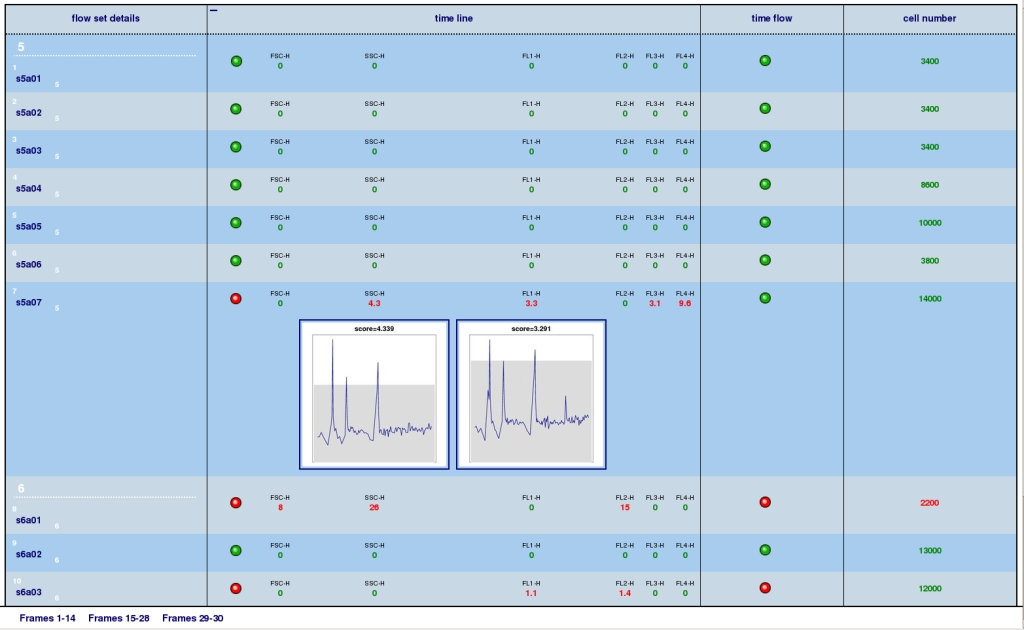
\includegraphics[width=0.75\textwidth]{flowQ.jpg}
\caption{\label{flowQ}% 
  HTML quality assessment report generated by
  the flowQ package. Rows correspond to samples, columns to different
  quality checks.}
\end{figure}

Static gating for all samples in a high-throughput FCM experiment is
often not an option, since the measured variables tend to vary between
different treatments, over time or between different experiment
batches. Automated or data-driven gating tries to estimate the gating
regions from the underlying data, thus providing a fast objective
solution to the analysis of potentially very large and diverse data
sets \cite{lo2008agf}. One of the automated gating methods implemented
in flowCore is based on identifying areas of significant curvature in
a kernel density estimate of the data \citep{wand2008}. Assuming that
the regions of interest are of high density, the software is able to
reliably detect them in a one or two-dimensional density landscape.

\begin{verbatim}
> cf <- curv2Filter("FL1-H", "FL3-H")
> fres <- filter(dat, cf)
\end{verbatim}

Kernel density estimation is a well-known problem in statistical
computing, and a lot of effort has been invested in the development of
good software to address it. The modular design of flowCore allows to
easily integrate these existing solutions into our framework. In this
example, we directly use R code from the feature package developed by
\cite{wand2008}. Instead of re-writing existing code, we are able to
include it via the well tested distribution mechanism provided by R's
software package system. This process is bi-directional, and all
functionality implemented in flowCore is available to other package
authors, as we have seen with the afore-mentioned flowClust package.

We can chose one of the many visualization option from the flowViz
package to plot the results of the recent filtering operation. A very
basic matrix of density plots is shown in Figure \ref{xyplot}, where
each panel in the matrix represents the data of one individual
patient.

\begin{verbatim}
> xyplot(`FL1-H` ~ `FL3-H` | SampleID, data=dat, filter=fres)
\end{verbatim}


\begin{figure}[htbp]
\centering
\includegraphics[width=0.75\textwidth]{xyplot}
\caption{\label{xyplot}%
Scatterplot matrix of a single flowSet with outlines of the gating
regions identified by an automated gating operation.}
\end{figure}



\section*{Discussion}

Through flowCore, we have provided the FCM community a freely
available, highly functional, standards compliant development and
analysis platform for high throughput data analysis.  Our intention is
to provide a platform for the collaborative development of new
analysis methods that will facilitate the transition of these new
methods to the larger flow community.  Our experience has been that the
collaborative effort we enable for devising new methodology has been
proven beneficial for a number of different biological and
computational biology challenges.  We hope that our framework will be
the foundation for fruitful shared research by many collaborators from
multiple scientific fields and will help resolve bottlenecks that
currently prevent the further development of and deployment of FC-HCS
to increasingly complex and important scientific and clinical
applications.

\section*{Acknowledgements}
This work was supported by NIH grant EB005034. RRB is a Michael Smith
Foundation for Health Research Scholar and a International Society for
Analytical Cytology Scholar.

\bibliographystyle{plainnat}  
\bibliography{flowCoreRef} 
\end{document}

